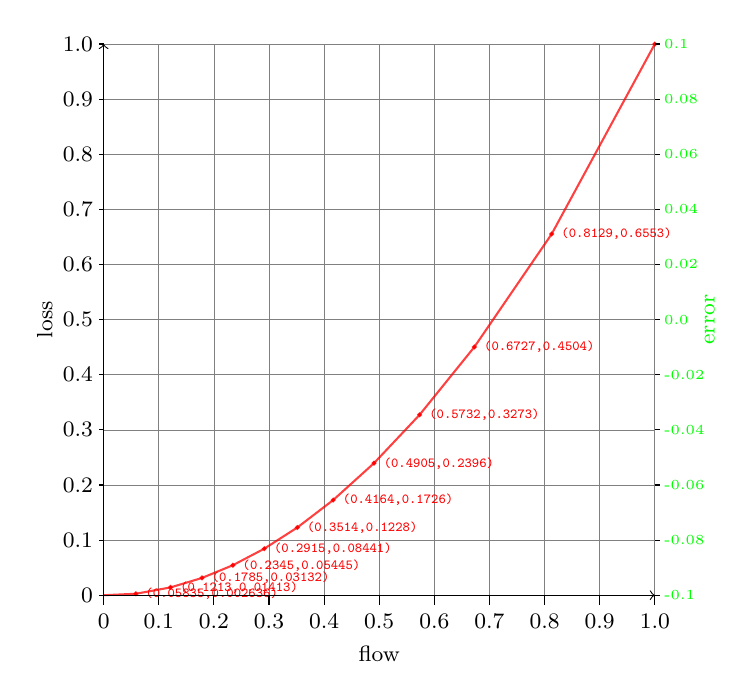
\begin{tikzpicture}[xscale=7.0,yscale=7.0]
\draw [help lines,step=0.1] (0,0) grid (1,1);
\filldraw[line width=0.5pt,color=blue!25!white,draw opacity=0.15,fill opacity = 0.5] plot file {txuse_12_hg.dat};
\draw[line width=0.5pt,color=black] plot file {txuse_12_XY.dat};
\coordinate (oneone) at (1,1);
\filldraw [red,draw opacity=0.75] (oneone) circle (0.1pt);
\coordinate (bk1) at (0,0);
\coordinate (bk2) at (0.058345,0.0026365);
\coordinate (bk3) at (0.12131,0.014128);
\coordinate (bk4) at (0.17848,0.03132);
\coordinate (bk5) at (0.2345,0.054455);
\coordinate (bk6) at (0.29151,0.084409);
\coordinate (bk7) at (0.35142,0.12285);
\coordinate (bk8) at (0.41644,0.1726);
\coordinate (bk9) at (0.49052,0.23957);
\coordinate (bk10) at (0.5732,0.32725);
\coordinate (bk11) at (0.67266,0.45041);
\coordinate (bk12) at (0.81286,0.65529);
\coordinate (bk13) at (1,1);
\filldraw [red,draw opacity=0.75] (bk2) circle (0.1pt) node[right] {\tiny \texttt{(0.05835,0.002636)}};
\filldraw [red,draw opacity=0.75] (bk3) circle (0.1pt) node[right] {\tiny \texttt{(0.1213,0.01413)}};
\filldraw [red,draw opacity=0.75] (bk4) circle (0.1pt) node[right] {\tiny \texttt{(0.1785,0.03132)}};
\filldraw [red,draw opacity=0.75] (bk5) circle (0.1pt) node[right] {\tiny \texttt{(0.2345,0.05445)}};
\filldraw [red,draw opacity=0.75] (bk6) circle (0.1pt) node[right] {\tiny \texttt{(0.2915,0.08441)}};
\filldraw [red,draw opacity=0.75] (bk7) circle (0.1pt) node[right] {\tiny \texttt{(0.3514,0.1228)}};
\filldraw [red,draw opacity=0.75] (bk8) circle (0.1pt) node[right] {\tiny \texttt{(0.4164,0.1726)}};
\filldraw [red,draw opacity=0.75] (bk9) circle (0.1pt) node[right] {\tiny \texttt{(0.4905,0.2396)}};
\filldraw [red,draw opacity=0.75] (bk10) circle (0.1pt) node[right] {\tiny \texttt{(0.5732,0.3273)}};
\filldraw [red,draw opacity=0.75] (bk11) circle (0.1pt) node[right] {\tiny \texttt{(0.6727,0.4504)}};
\filldraw [red,draw opacity=0.75] (bk12) circle (0.1pt) node[right] {\tiny \texttt{(0.8129,0.6553)}};
\draw[line width=0.75pt,color=red,draw opacity=0.75] (bk1) -- (bk2); 
\draw[line width=0.75pt,color=red,draw opacity=0.75] (bk2) -- (bk3); 
\draw[line width=0.75pt,color=red,draw opacity=0.75] (bk3) -- (bk4); 
\draw[line width=0.75pt,color=red,draw opacity=0.75] (bk4) -- (bk5); 
\draw[line width=0.75pt,color=red,draw opacity=0.75] (bk5) -- (bk6); 
\draw[line width=0.75pt,color=red,draw opacity=0.75] (bk6) -- (bk7); 
\draw[line width=0.75pt,color=red,draw opacity=0.75] (bk7) -- (bk8); 
\draw[line width=0.75pt,color=red,draw opacity=0.75] (bk8) -- (bk9); 
\draw[line width=0.75pt,color=red,draw opacity=0.75] (bk9) -- (bk10); 
\draw[line width=0.75pt,color=red,draw opacity=0.75] (bk10) -- (bk11); 
\draw[line width=0.75pt,color=red,draw opacity=0.75] (bk11) -- (bk12); 
\draw[line width=0.75pt,color=red,draw opacity=0.75] (bk12) -- (bk13); 
\draw[->] (0,0) -- node[midway,yshift=-0.75cm] {\footnotesize flow} (1,0);
\draw[->] (0,0) -- node[rotate=90,midway,yshift=0.75cm] {\footnotesize loss} (0,1) ;
\foreach \x/\xtext in {0,0.1,0.2,0.3,0.4,0.5,0.6,0.7,0.8,0.9,1.0}
\draw (\x cm,0pt) -- (\x cm,-0.5pt) node[anchor=north] {\footnotesize \xtext};
\foreach \y/\ytext in {0,0.1,0.2,0.3,0.4,0.5,0.6,0.7,0.8,0.9,1.0}
\draw (0.0pt,\y cm) -- (-0.25pt,\y cm) node[anchor=east,xshift=0.5mm] {\footnotesize \ytext};
\draw[line width=0.5pt,color=green,draw opacity=0.75] plot file {txuse_12_err.dat};
\foreach \y/\ytext in {0/-0.1,0.1/-0.08,0.2/-0.06,0.3/-0.04,0.4/-0.02,0.5/0.0,0.6/0.02,0.7/0.04,0.8/0.06,0.9/0.08,1.0/0.1}
\draw (1cm,\y cm) -- (1.01cm,\y cm) node[anchor=west,xshift=-0.75mm] {\tiny \textcolor{green}{\ytext}};
\node[rotate=90] at (1.1,0.5) {\footnotesize \textcolor{green}{error}};
\end{tikzpicture}
